\chapter{REVISIÓN DE LITERATURA}
\section{Definición de términos clave}

\begin{definition}[Monitoreo]
  El monitoreo es un proceso sistemático y continuo que permite observar, registrar y analizar parámetros específicos para evaluar el estado o cambios en un sistema o fenómeno determinado. Es fundamental para la toma de decisiones informadas en la gestión ambiental y otros campos. \cite{ciga_monitoreo}
\end{definition}


\begin{definition}[Ciencia Ciudadana]
La ciencia ciudadana es una metodología científica que involucra activamente a la ciudadanía en la generación de conocimiento, permitiendo que personas sin formación científica formal participen en la recolección, análisis e interpretación de datos, contribuyendo así a proyectos de investigación y al fomento de la cultura científica.\cite{csic_ciencia_ciudadana}
\end{definition}




\begin{definition}[Flutter]

Flutter es un framework de código abierto desarrollado por Google que permite crear aplicaciones nativas de alto rendimiento para múltiples plataformas (iOS, Android, web, escritorio) a partir de una única base de código, utilizando el lenguaje de programación Dart.\cite{flutter_multiplataforma}
\end{definition}

\begin{definition}[Dart]

Dart es un lenguaje de programación desarrollado por Google, diseñado para crear aplicaciones frontend rápidas y optimizadas, especialmente utilizado en conjunto con Flutter.
\end{definition}
\begin{definition}[Firebase]

Firebase es una plataforma de desarrollo de aplicaciones creada por Google que proporciona servicios como bases de datos en tiempo real, autenticación de usuarios, hosting de archivos y funciones de backend sin servidor, facilitando el desarrollo y escalamiento de aplicaciones móviles y web.
\end{definition}


\begin{definition}[Backend]
El backend se refiere a la parte del desarrollo de software que gestiona la lógica de negocio, bases de datos, servidores y APIs, funcionando como la estructura interna que sostiene y conecta los servicios de una aplicación.
\end{definition}






\begin{definition}[Firebase Realtime Database]
Es un servicio de base de datos en la nube que almacena y sincroniza datos entre usuarios en tiempo real, ideal para aplicaciones que requieren actualizaciones inmediatas.
\end{definition}
















\begin{definition}[Pluviómetro manual]

El pluviómetro manual es un instrumento utilizado para medir la cantidad de precipitación líquida caída en un lugar específico durante un período determinado. Consiste en un recipiente cilíndrico que recoge el agua de lluvia, la cual se mide posteriormente con una probeta graduada. Este instrumento debe cumplir con las especificaciones establecidas en las normas mexicanas para garantizar la precisión y confiabilidad de los datos obtenidos.\cite{semarnat_pluviometro}
\end{definition}

Las especificaciones para construir un pluviómetro, ilustradas en la figura \ref{t1}, son:
\begin{itemize}
    \item El depósito debe tener una entrada estrecha, suficientemente protegida de la radiación, para reducir al mínimo las pérdidas de agua por evaporación
    \item Este instrumento debe colocarse en lugares abiertos y su área de captación debe permanecer horizontal y a 100 cm del suelo. \cite{se2013}
\end{itemize}

\begin{figure}[ht]
\centering
  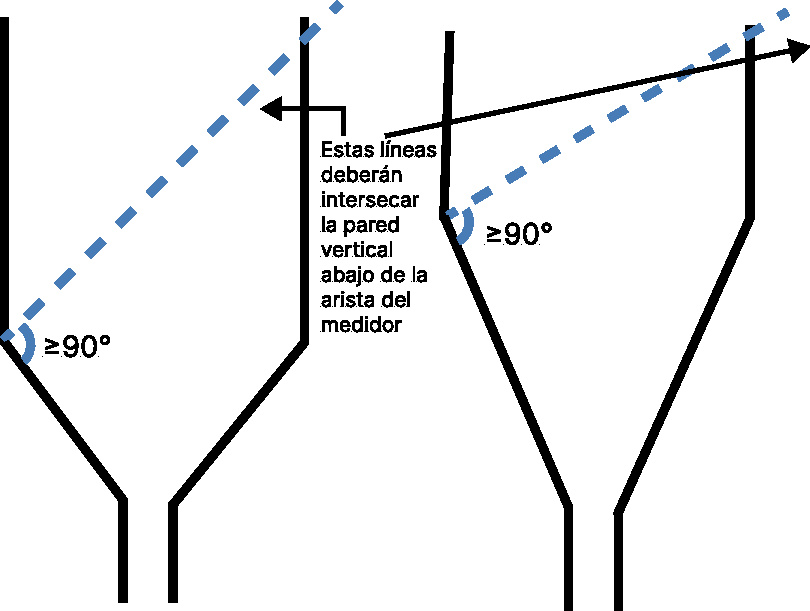
\includegraphics[width=0.5\textwidth]{t1.pdf}
  \caption{Colectaros adecuados para los pluviómetros. (NORMA MEXICANA, 2013)}
  \label{t1}
\end{figure}

















\section{Acceso a datos meteorológicos  de zonas de montaña en México}

\section{Revisión de estudios previos sobre monitoreo ciudadano meteorológico}

\section{Tecnologías actuales en monitoreo climático}

IMPORTANCIA HIDROLÓGICA DE LAS ZONAS DE MONTAÑAS

\section{Aportes del monitoreo ciudadano a la ciencia climática}









